\documentclass{standalone}
\usepackage{tkz-fct}
\usepackage{amsmath}
\usepackage{tkz-tab}
\usepackage{tkz-euclide}
\usepackage{color}
\newcommand{\vect}[1]{\overrightarrow{#1}}

\renewcommand*\familydefault{\sfdefault}
\usepackage{sansmath}
\sansmath
\definecolor{gray75}{gray}{0.75}
\begin{document}

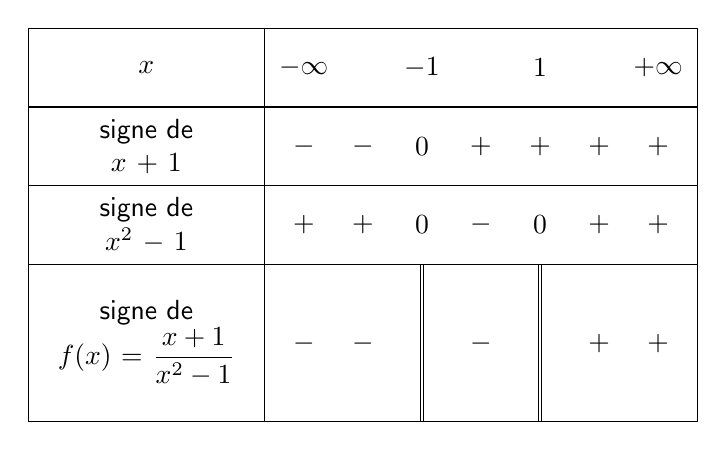
\begin{tikzpicture}
  \tkzTabInit[espcl=1.5, lgt=3]%
  {$x$ / 1,signe de\\ $x+1$ / 1, signe de\\$x^{2}-1$/1, signe de\\$f(x)=\dfrac{x+1}{x^{2}-1}$/2}%
  {$-\infty$,$-1$,$1$,$+\infty$}%
  \tkzTabLine{-,-,0,+,+,+,+}
  \tkzTabLine{+,+,0,-,0,+,+}
  \tkzTabLine{-,-,d,-,d,+,+}

\end{tikzpicture}

\end{document}
 % Local Variables:
 % TeX-command-extra-options: "-shell-escape"
 % End:
